\section{System Overview}
\label{sec:overview}
% of a Real-time Traffic Map}


\begin{figure}[t!]
\centering
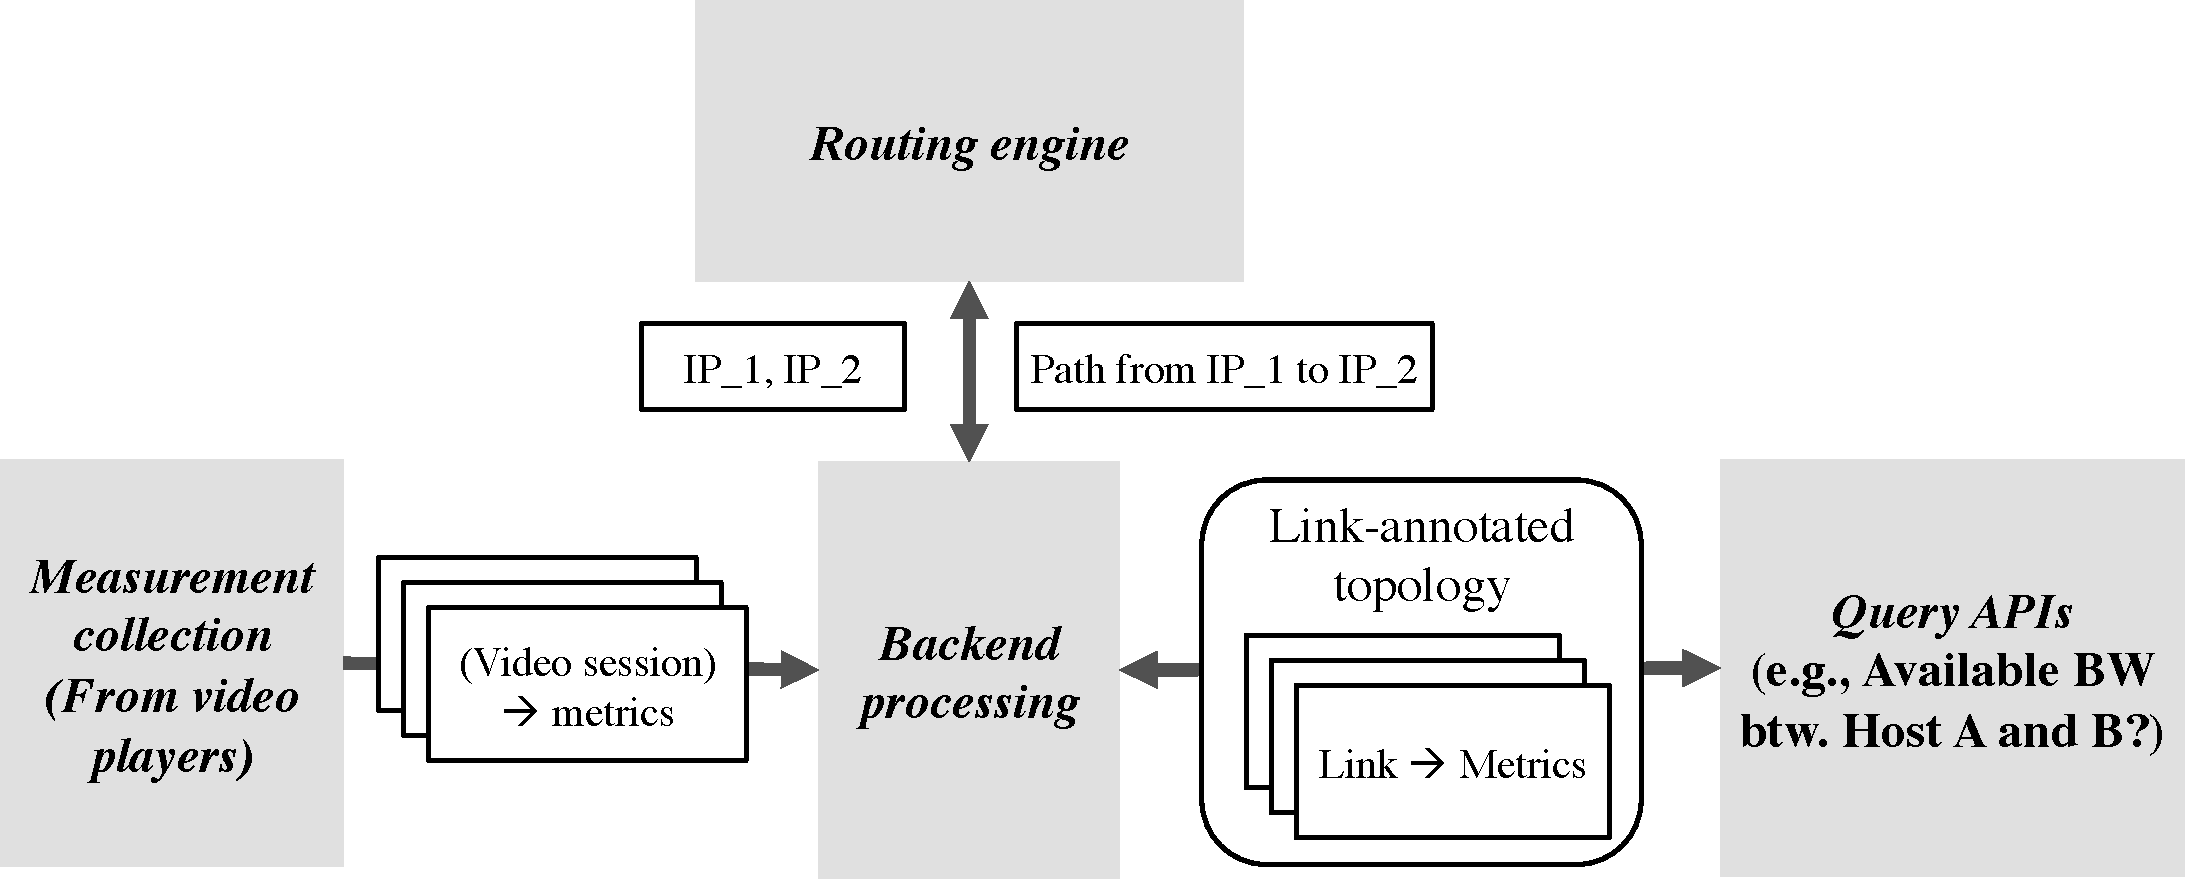
\includegraphics[width=230pt]{figures/system_overview_short.pdf}
\vspace{-0.3cm}
\tightcaption{High level components a Real-time Traffic Map. The {\it measurement engine} gathers raw data of application-layer metrics (e.g., download speed) from client-side video players, and then the {\it backend processing} combines the performance between server and client with their paths obtained by looking up the {\it routing engine} to generate a link-annotated graph. The link-annotated graph can be used to predict answer {\it query APIs} such as bandwidth between two given hosts.}
\label{fig:overview:system}
\end{figure}

Our overarching vision is to create a {\em  Real-time Traffic Map (RTM)}
 as shown in Figure~\ref{fig:overview:system}. The RTM is a
service that applications can query using a public API to obtain a near
real-time available bandwidth estimate between arbitrary pairs of end hosts.
 The key enabler  is to use the massive video-based measurements collected 
  to obtain a simultaneous and collective view over the Internet with
a great coverage offered by the video traffic.  These  measurements 
 are used in conjunction with other routing engines such as 
 iPlane to ultimately a generate an annotated topology map for the 
 Internet.

 
As discussed earlier, such a service can benefit many distributed applications.
For example, CDN re-direct client requests to edge servers based on the
performance predicted between the client and servers with the replica of
requests. Likewise, many of today's video players~\cite{hds,netflix} request
content dynamically from multiple CDNs.  Peer-to-peer file distribution and
overlay multicast can benefit from peer-selection based on real-time
information of available bandwidth between two hosts. 

%What RTM provides is the technique base for building up such service. In reality, 


We envision different operational models  for such a service in practice.   Our
vision is broad enough and the RTM can be operated by different entities who
have access to video player performance.  These include video content
providers, CDN, or third-party companies. And it has been shown feasible as
some companies (e.g., Akamai) have been collecting performance characteristics
from video players for different purposes. The coverage of the RTM service
operated by different parties may depend on their visibility -- for example,
CDNs have the view of all traffic from its own servers, while content provider
may leverage the opportunities of using multiple CDNs to obtain a different
visibility. As such our focus in this paper is on establishing the technical
basis for such an RTM rather than the economics or service-level aspects.

Unlike existing systems such iPlane which leverages on a few fully controlled
nodes to carry out fine-grain (packet-level) probing and measurement, we measure
the video traffic from the view of massive video players to collect bandwidth
information. However, this poses new challenges in two aspects.

\mypara{Coarse measurement} While our approach achieves better coverage, the
measured bandwidth between two hosts will be in much more coarse-grain, because
the video players run within the browser sandbox in  application-layer and have
little knowledge of packet-level statistics. This means the bandwidth will be
measured over a coarser time duration than that of packet dispersion techniques like
Spruce~\cite{strauss2003measurement}, IGI~\cite{hu2003evaluation}.  Moreover, caching effect also
impacts the measured bandwidth, since CDNs often fetch video content from
different servers or even from a local copy.

\mypara{End-to-end measurement} Because of the sandbox limitation, it is
infeasible to collect path information by traceroute video players. So it is
challenging to predict the bandwidth between two hosts that have never been
probed by video traffic. For example, we can have bandwidth information between
each of two clients and a server, but it is very likely that the two clients
have never been probed from one to another.


\mypara{Near real-time response} Instead of managing updates from a few
machines, our approach has to handle concurrent client-side measurement from
millions of video viewers, maintain the most up-to-date information of paths
and links, and process a large number of queries in nearly real-time. We
postpone the discussion of scalability issues to Section~\ref{sec:disc}.


Ideally, like iPlane, to predict available bandwidth between hosts that have never been probed, RTM can adopt the idea of structural prediction in which
a link-annotated map is first generated and the prediction of path performance
is made by composing the segments (e.g., links) pre-calculated on the map. To
this end, we have to first identify the path which each end-to-end measurement
is using. Several existing systems provide such service; e.g., 
iPlane predicts current IP level route between any two hosts by
concatenating paths observed in traceroute data. 

With the path information, the measured metrics
associated to paths need to be converted to metrics associated to more basic
composable unit (i.e., link) which can be later composed to predict metrics of
a path that may have never been probed before.

This is challenging since we receive only application-level bandwidth
measurement. However, we can compensate the coarse-grain input with the massive
simultaneous vantage view of video traffic. The high-level idea is to combine
the routing information and bandwidth measurement using some extrapolation logic
that exploits the correlation of the massive simultaneous probes from different
paths to obtain link-level information. We present the technique in the next section.
